\documentclass[a0paper,portrait]{baposter}
\usepackage{wrapfig}
\usepackage{lmodern}
\usepackage[utf8]{inputenc} %unicode support
\usepackage[T1]{fontenc}
\usepackage{amsmath}
%\selectcolormodel{cmyk}
\usepackage{relsize}		% For \smaller
\usepackage{url}			% For \url
\usepackage{epstopdf}	% Included EPS files automatically converted to PDF to include with pdflatex
\usepackage{amsmath}
\usepackage{multicol}
\usepackage{graphicx}
\usepackage{tcolorbox}
\usepackage{wrapfig}

\graphicspath{{figures/}} % Directory in which figures are stored
\newcommand{\compresslist}{%
\setlength{\itemsep}{0pt}%
\setlength{\parskip}{1pt}%
\setlength{\parsep}{0pt}%
}
\newenvironment{boenumerate}
  {\begin{enumerate}\renewcommand\labelenumi{\textbf\theenumi.}}
  {\end{enumerate}}
\begin{document}

%\definecolor{darkgreen}{cmyk}{0.14,0.13,0.8,0.18}
%\definecolor{lightblue}{cmyk}{0.8,0,0.8,0.25}
\begin{poster}
{
grid=false,
headerborder=open, % Adds a border around the header of content boxes
colspacing=1em, % Column spacing
bgColorOne=white, % Background color for the gradient on the left side of the poster
bgColorTwo=white, % Background color for the gradient on the right side of the poster
borderColor=green, % Border color
headerColorOne=green, % Background color for the header in the content boxes (left side)
headerColorTwo=black, % Background color for the header in the content boxes (right side)
headerFontColor=white, % Text color for the header text in the content boxes
boxColorOne=white, % Background color of the content boxes
textborder=rounded, %rectangle, % Format of the border around content boxes, can be: none, bars, coils, triangles, rectangle, rounded, roundedsmall, roundedright or faded
eyecatcher=false, % Set to false for ignoring the left logo in the title and move the title left
headerheight=0.11\textheight, % Height of the header
headershape=rounded, % Specify the rounded corner in the content box headers, can be: rectangle, small-rounded, roundedright, roundedleft or rounded
headershade=plain,
headerfont=\Large\textsf, % Large, bold and sans serif font in the headers of content boxes
%textfont={\setlength{\parindent}{1.5em}}, % Uncomment for paragraph indentation
linewidth=2pt % Width of the border lines around content boxes
}
{}
%
%----------------------------------------------------------------------------------------
%	TITLE AND AUTHOR NAME
%----------------------------------------------------------------------------------------
%
{
\textsf %Sans Serif
{Energy landscape of a designed protein, a shallow trefoil knot and a deep trefoil knot
}
}
{\sf\vspace{0.2em}\\
Sridhar Neelamraju$\dagger$$\ddagger$, Shachi Gosavi$\dagger$ and David Wales$\ddagger$
\vspace{0.1em}\\
\small{$\dagger$National Centre for Biological Sciences, Bangalore, India $\ddagger$ University Chemical Laboratories, Lensfield Road, University of Cambridge, UK.
\vspace{0.2em}}
}
{
\includegraphics[height=0.5in, width=1in]{logo_ncbs.jpg}} % University/lab logo
	

\headerbox{1. Introduction}{name=introduction,column=0,row=0, span=3}{Proteins designed artificially have not had the benefit of evolution and are typically designed only to stabilise the native state. Natural proteins, on the other hand, have evolved to function as well as fold, and this is a likely source of  frustration. We study the potential energy landscapes of Top7, a model designed protein and S6, a natural protein of comparable size, using a combination of molecular dynamics (MD) and discrete path sampling (DPS)\cite{Neelamraju17a, Truong} and quantify the frustration resulting from the designed topology of Top7 with a frustration density parameter.   

Topological frustration is particularly evident in knotted proteins. In order to avoid the common problstrem of chain-crossings that result for C$\alpha$ coarse-grained description, the doubly-nudged elastic band scheme (DNEB) is enhanced with Quasi-Continuous Interpolations (QCI) for coarse-grained structure-based models (SBMs). This allows us to find paths connecting distant conformations that are usually difficult to find with molecular dynamics alone. As an example, we construct kinetic transition networks for three different trefoil knots: MJ0366 (a trefoil knotted protein explored extensively in the past with MD), 1mxiS (a shallow trefoil knot formed by the truncated protein YibK) and 1mxiD (a deep trefoil knot formed by truncated protein YibK). The resulting kinetic transition network identifies topological traps along the potential energy landscapes of each of the three proteins studied. Further, in each case, we identify how high above the native state the process of knotting begins through application of a knot detection algorithm.}

\headerbox{Structure Based Models}{name=gokit,column=0,below=introduction,span=2}{
\begin{equation}


\begin{aligned}
U = &
\sum_{i=1,N-1}\frac{K_b}{2}\big(r_i-r_O\big) + \sum_{i=1,N-2}K{_\theta} \big( \theta _i - \theta_O\big )  + \sum_{i=1,N-3}\frac{K_{\phi}}{2}\big( 1-cos\big( 2\phi_i - \frac{\pi}{2}\big)\big) \\ 
  & +\sum_{i<j-3}^{Nat-C}\epsilon_{ij}\Big[5\Big( \frac{\sigma_{ij}}{r_{ij}}\Big)^{12} - 6\Big( \frac{\sigma_{ij}}{r_{ij}}\Big)^{10}  \Big] + \sum_{i<j-3}^{Non-C}\epsilon_{ij}\Big(\frac{C}{r_{ij}}\Big)^{12}
  \label{eq:eq1}
\end{aligned}
\end{equation}
Artificial frustration is added with introducing non-native interactions among hydrophobic residues. 
Effect of water molecules with a desolvation barrier potential\cite{Chan}. Effect of side-chain interactions with a statistical two-bead Cheung-Thirumalai potential\cite{Cheung}. See Gokit\cite{Neelamraju19a} for applying model to single domain proteins.}
% \headerbox{2.Energy Landscape representations}{name=screen,span=1,column=2,below=introduction}{
% \includegraphics[width=0.9\textwidth]{schematic.png}\\
% Pictorial correspondence between a potential energy landscape and a disconnectivity graph following Becker and Karplus[4].(Top) A funnelled landscape is represented by a single stem (Palm-tree). A glassy energy landscape(bottom) is represented by multiple stems (Banyan tree). \\
% \vspace{4pt}
% }

\headerbox{Top7 Vs S6:Molecular Dynamics}{name=Top7,column=0, span=1, below=gokit}{ % To reduce this block to 1 column width, remove 'span=2'
\begin{center}
\includegraphics[width=0.8\linewidth]{S6_Top7.png} \\
\end{center}
In keeping with literature, no intermediates are found for the naturally evolved S6 protein while the free-energy landscape for Top7 shows distinct intermediates while folding with different flavours of coarse-grained Structure-Based Models.. 
}

\headerbox{Top7 Vs S6:Discrete Path Sampling}{name=Top7DPS,column=1, span=1, below=introduction}{ % To reduce this block to 1 column width, remove 'span=2'
\begin{center}
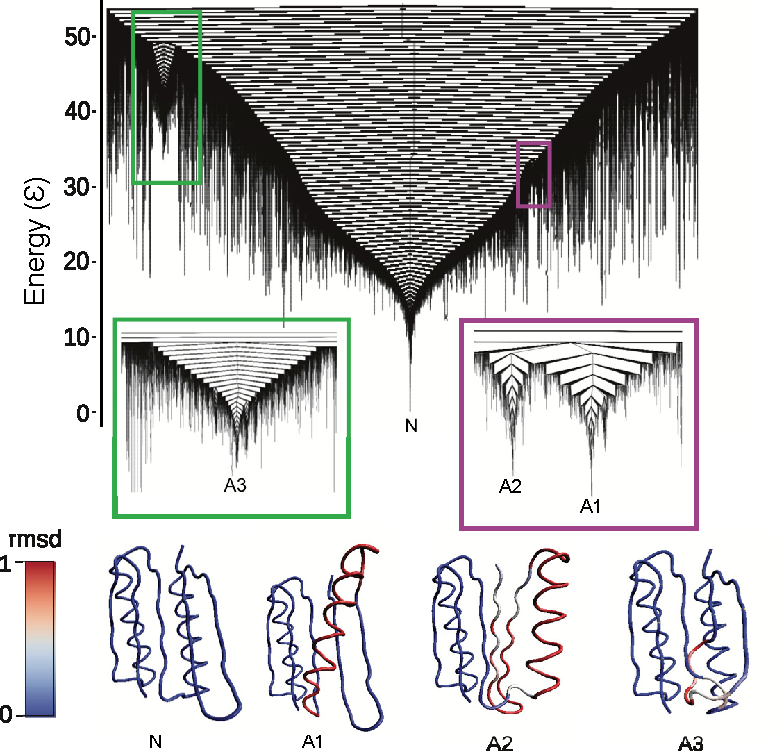
\includegraphics[width=0.8\linewidth]{tree4_5.pdf} \\    
\end{center}
Disconnectivity graph representation of the ensemble of stationary points derived with DPS for the 4.5~\AA~cut-off contact map. Blue indicates the parts of the protein similar to the native state (N) and red indicates a high RMSD difference obtained from an RMSD-based per residue structural alignment.
}
\headerbox{Top7 Vs S6: Frustration Density}{name=Top7frust,column=2, span=1, below=introduction}{ % To reduce this block to 1 column width, remove 'span=2'
\begin{center}
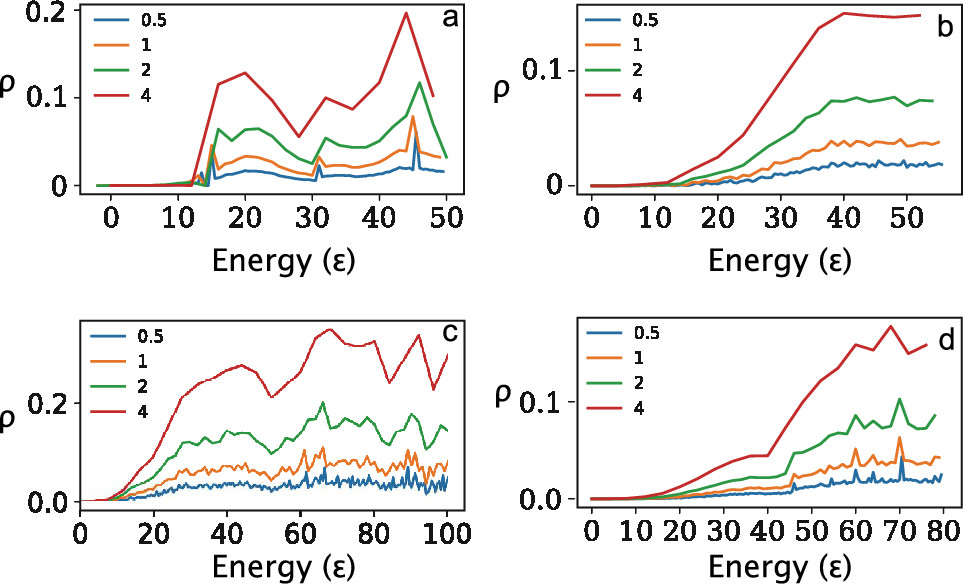
\includegraphics[width=\linewidth]{frustrationdensity.jpeg} \\
\end{center}
Frustration density, $\rho$, as a function of the energy interval for the disconnectivity graphs at $\delta$=0.5$\varepsilon$ (blue), 1$\varepsilon$ (orange), 2$\varepsilon$ (green) and 4$\varepsilon$ (red) . (a) Top7 - C$\alpha$ model, (b) S6 - C$\alpha$ model, SCM-based map, (c) Top7 - C$\alpha$-C$\beta$ model and (d) M7- C$\alpha$ model. The horizontal axis is scaled to δ=1$\varepsilon$. 
For the Top7, a funnelled structure-based model representation shows distinct fluctuation in the frustration density parameter. These fluctuations are absent for S6 and M7}
\headerbox{MJ0366: A simple trefoil knot}{name=MJ0366,column=0, span=1, below=Top7}{

\begin{center}
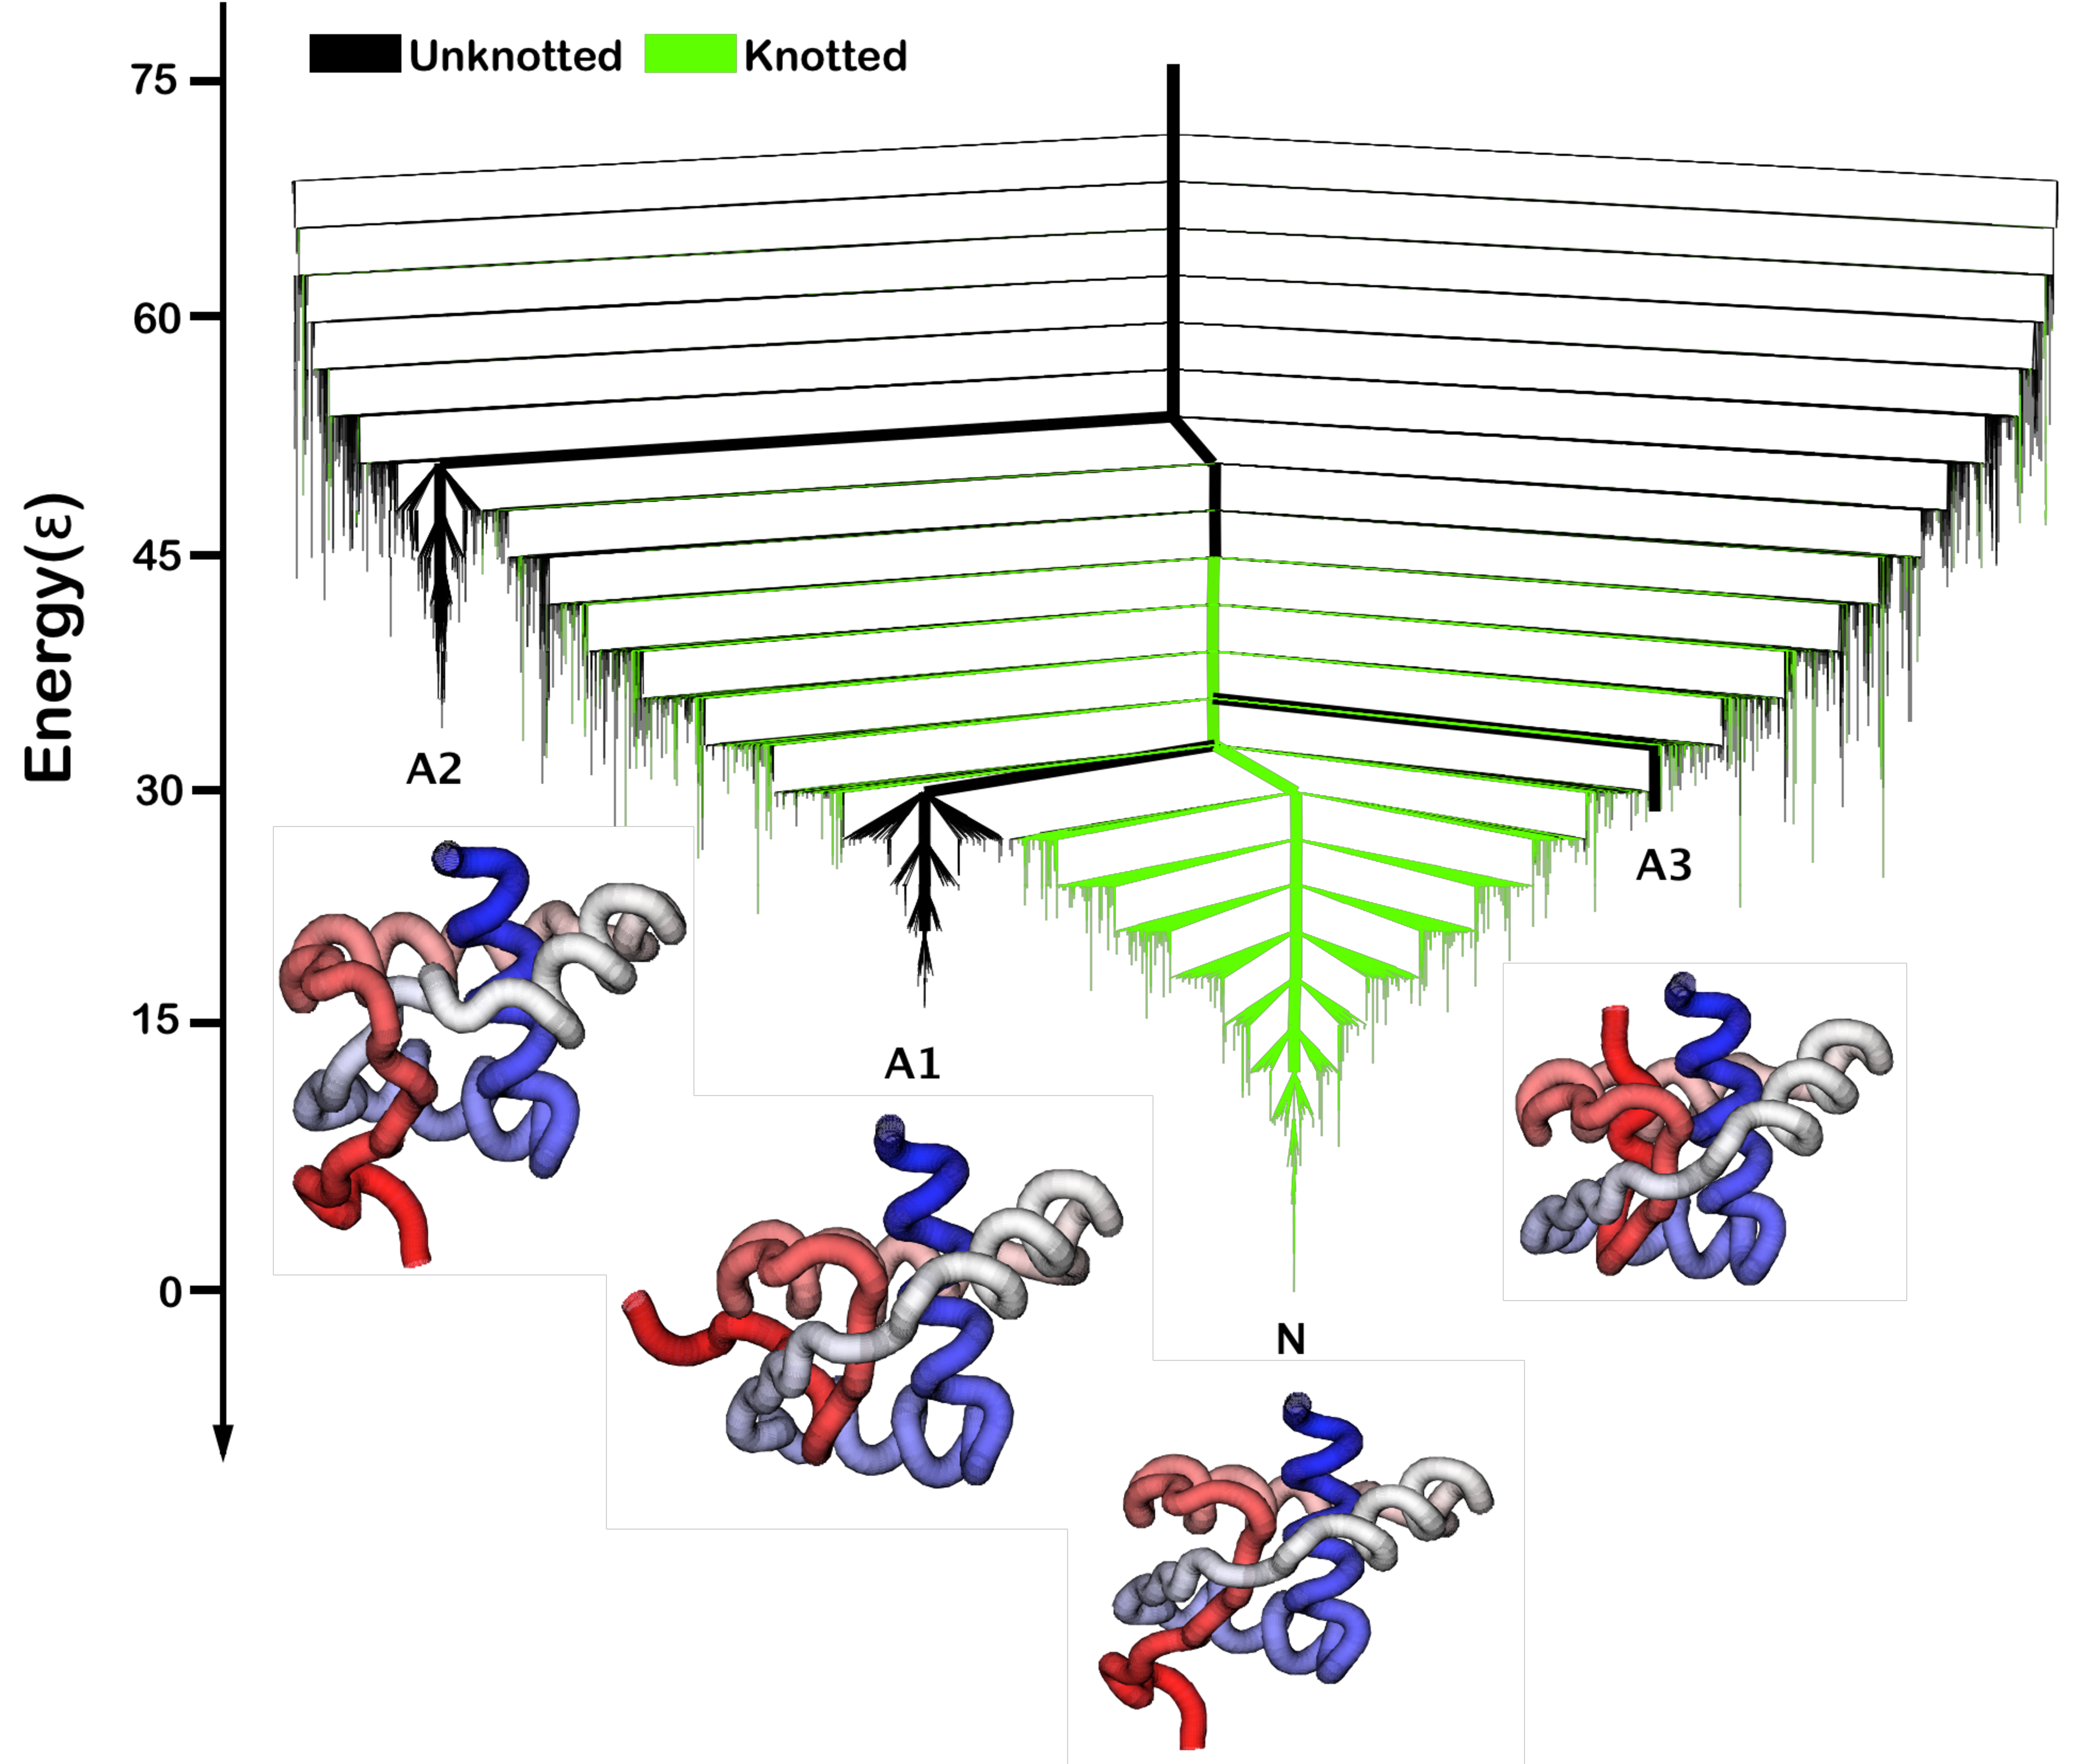
\includegraphics[width=\linewidth]{MJ0366.pdf} 
\end{center}
Text about many previous MD runs. What's new here? Estimate of topological barriers, At what point knotting begins? etc. 
}

\headerbox{HI0766: Deep Vs Shallow  trefoil knots}{name=HI0766,column=1, span=2, below=Top7DPS}{

\begin{center}
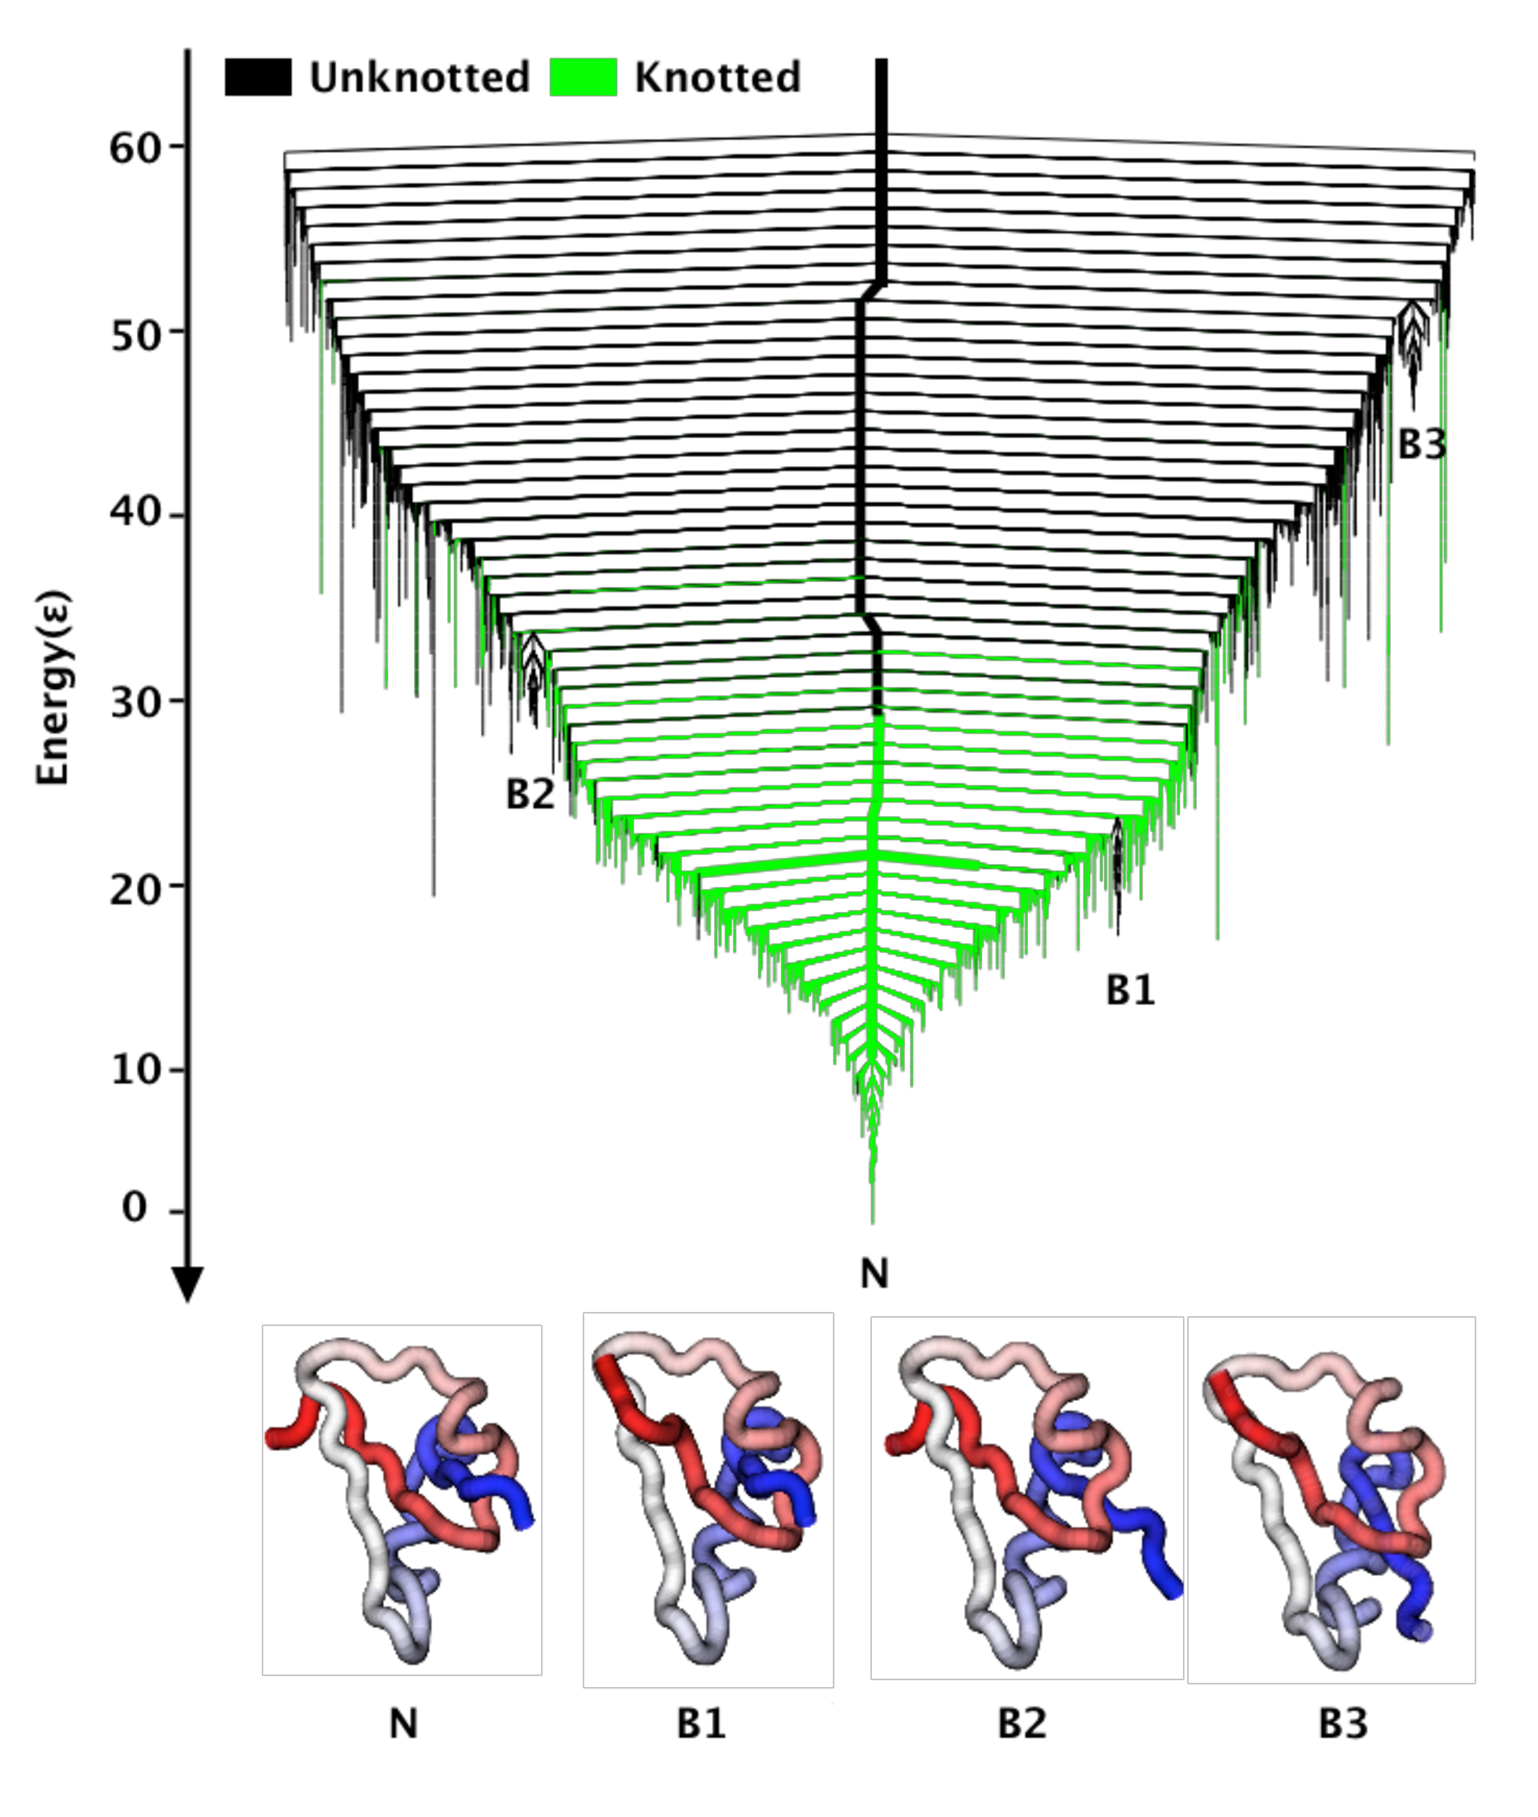
\includegraphics[width=0.5\linewidth]{1mxi5_tree.pdf} 
\end{center}
Text about many previous MD runs. What's new here? Estimate of topological barriers, At what point knotting begins? etc. 
}







% \headerbox{5. Top7 Vs S6: DPS}{name=dps,column=1, span=2, below=sbm}{ % To reduce this block to 1 column width, remove 'span=2'
% \begin{center}
% \includegraphics[width=\linewidth]{top7_tree.png}\\
% \end{center}
% A database of connected stationary points is derived from DPS. This is visualised as a disconnectivity graph. (a) A small kinetic trap found for Top7 with a C$\alpha$-SBM (4.5~\AA~ cutoff). (b) Adding non-native attractive hydrophobic interactions leads to narrowing of the funnel. (c) A fully funnelled disconnectivity graph derived for the naturally evolved S6 protein with a C$\alpha$-SBM.

% \begin{center}
% \includegraphics[width=0.6\linewidth]{conprob.png}\\
% \end{center}
% % Probability of formation of each contact on a contact-map derived from an ensemble of low-lying minima around the native-state derived from DPS. (a) C$\alpha$-SBM (4.5~\AA~), (b) C$\alpha$-SBM (6.5~\AA~) and (c)C$\alpha$-SBM (4.5~\AA~)+hydrophobic interactions. Addition of hydrophobic interactions destabilises the N-terminal region considerably.}

% \headerbox{6. Conclusions and Outlook}
% {name=references,column=0,span=1,below=md,above=bottom}{

% %\small % Reduce the font size in this block
% \renewcommand{\section}[2]{\vskip 0.05em} 
% \begin{boenumerate}\compresslist
% \item {DPS can be used to explore the energy landscapes of complex biomolecules like designed proteins.}
% \item{Proteins described by an all-atom AMBER potential can also be studied with the help of GPUs to predict energetic barriers, rate-constants and likely pathways for conformational transitions.
% \item{The chemical basis for kinetic trapping can be elucidated followed by informed mutations that might help sculpt a smooth energy landscape for designed proteins}

% \vspace{5pt}
% }

% \end{boenumerate}

% }

% \headerbox{7 References}
% {name=references,column=1,span=2,below=dps,above=bottom}{
% \small % Reduce the font size in this block
% \renewcommand{\section}[2]{\vskip 0.05em} % Get rid of the default "References" section title
% %\nocite{*} % Insert publications even if they are not cited in the poster
% [1] Liu and Chan, J. Mol. Biol. 349(4);872-889, 2005.[2] Cheung and Onuchic, J. Phys. Chem. B, 107(40):11193-11200,2003. [3] http://www-wales.ch.cam.ac.uk/PATHSAMPLE.[4] Becker and Karplus. J. Chem. Phys.,106(4):1495-1517,1997.,[5] Truong and Wolynes,J. Chem. Phys 139(12):121908,2013.
% }









\end{poster}

\end{document}
